\documentclass[article, a4paper, 12pt]{article}
\usepackage[brazil]{babel} %linguagem do documento
\usepackage[utf8]{inputenc} %reconhece acento e cedilha
\usepackage[top=3cm,left=2.5cm,right=2.5cm,bottom=2cm]{geometry} %margens
\usepackage{setspace}
%\usepackage{bbm.sty}
\usepackage{graphicx,url}
\thispagestyle{empty}
% coloracao
\usepackage{hyperref}
\hypersetup{
	colorlinks=true,
    urlcolor=blue,
    linkcolor=black
}

\begin{document}
	\onehalfspacing	
	\begin{center}
		\large{\textbf{INF628 - Estratégias de Busca em Inteligência Artificial}} \\
		\Large{Relatório Trabalho 2 \\ Algoritmo Genético}
	\end{center}
	\begin{large}
		\textbf{Aluno:} Michael Canesche \hspace{2cm} \textbf{Matrícula:} 68064 \\ \textbf{Prof.:} Levi Lelis \hspace{4cm} \textbf{Data de entrega:} 06/05/2019
	\end{large}


\section{Informações essenciais}

O código fonte pode ser encontrado no github pelo link: 

$\cdot$ \url{https://github.com/canesche/robot-openAI-genectic}

\subsection{Dependências}

A versão utilizada do python foi a 3.6.7, mas é totalmente replicável para as versões mais recentes.\\
O comando abaixo é para instalar as dependências (caso seja necessário).

$\cdot$ \textit{pip3 install --user -r requirements.txt}

\subsection{Como rodar}

Para executar o código basta utilizar o comando abaixo:

$\cdot$ \textit{python3 main.py}\\
Para executar o melhor indíviduo gerado:

$\cdot$ \textit{python3 main.py data$\backslash$individualbest.txt}

\section{Sobre o trabalho}

\hspace{1cm}O objetivo do trabalho é fazer com que o robô bípede (Figura \ref{fig:robotbegin}) aprenda a andar por um caminho que muda ligeiramente a cada interação, utilizando como algoritmo de aprendizagem o algoritmo genético. O robo é controlado pelas ações dos joelhos e as duas juntas do quadril, sendo essas ações valores que variam dentre -1 a 1, nos quais são respectivamente as velocidades angulares do joelho 1, quadril 1, joelho 2, quadril 2. Além disso, o ambiente oferece também observações feitas pelos sensores do robo, no qual não foi utilizado nesse trabalho.

\begin{figure}[!htb]
     \centering
     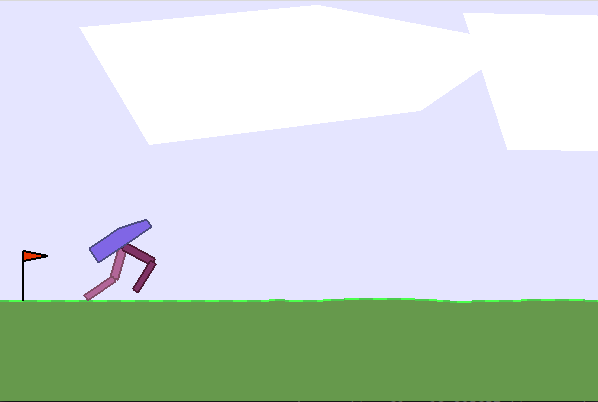
\includegraphics[scale=0.5]{img/robot_begin.png}
     \caption{Robô bípede no cenário}
     \label{fig:robotbegin}
\end{figure}

\section{Solução proposta}

\hspace{1cm}Abaixo tem uma abordagem de como foi modelado o problema: \\

$\cdot$ \textbf{Gene ou Ação}: vetor de tamanho 4, definido pelos valores derivados pelos joelhos e dos quadris.

$\cdot$ \textbf{Individuo}: Conjunto de ações ou conjunto de genes. No trabalho foi definido um valor constante de 16 ações. Esse valor foi escolhido empiricamente devido aos resultados obtidos pela função de adaptação.

$\cdot$ \textbf{População}: Conjunto de 100 indíviduos. Esse valor foi escolhido por ser mais do que suficiente para gerar uma boa população. 

$\cdot$ \textbf{Seleção}: O algoritmo de seleção utilizado foi o torneio aleatório, no trabalho é selecionado 10 indíviduos aleatórios e dentre eles é selecionado o melhor.

$\cdot$ \textbf{Crossover}: Nessa etapa foi selecionado uma parte de tamanho aleatório e a partir desse tamanho é trocado por entre os dois indivíduos. Criando-se assim dois filhos que vieram da combinação dos pais.

$\cdot$ \textbf{Mutação}: Enfim, foi criado um grupo elite, no qual é formado pelos melhores (20 indivíduos) da atual geração. Eles possuem a probabilidade de serem gerados uma probabilidade para verificarem se serão mutados ou não em seus genes. Além disso, foi criado um hall da fama, sendo eles os melhores dos melhores das gerações e eles são sempre passados para as próximas gerações. Note que esses 5 super individuos tem a probabilidade de serem mutados, o fato aqui de usar esse artíficio é para que não percam os seus genes caso a próxima geração seja pior do que a anterior.

\section{Resultados obtidos}

\hspace{1cm}Na figura \ref{fig:melhor}, temos o melhor resultado dentre várias épocas considerando o número máximo de 500 passos pelo robô. Note que é vísivel vê o crescimento da função de adaptação ao passar as gerações e que seu maiores crescimentos foram em torno das gerações 20 á 40 e da gerações 70 á 80. No qual, seu valor máximo de fitness é na geração 79 com o valor de aproximadamente 45.   

\begin{figure}[!htb]
     \centering
     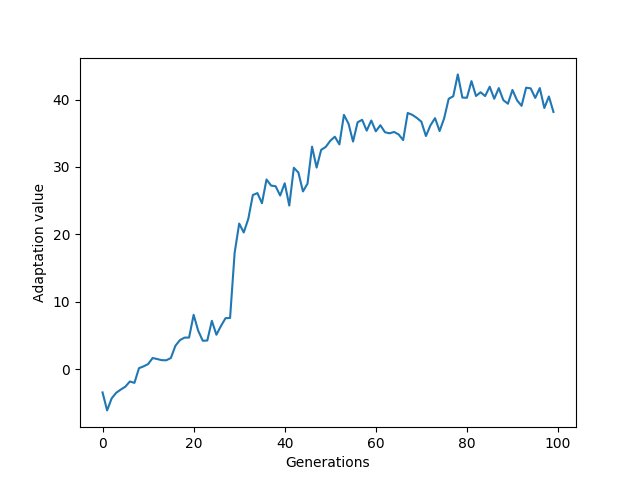
\includegraphics[scale=0.75]{img/melhor.png}
     \caption{Melhor resultado obtido dentre várias épocas}
     \label{fig:melhor}
\end{figure}

\hspace{0.5cm}Do resultado acima, a melhor maneira como o robô "aprendeu" a andar foi se impulsonando com um dos joelhos e o outro joelho é utilizado para ser estabilizado no ambiente (Figura \ref{fig:robotwalk}). Aparentemente outras formas de andar pelo robô (e.g. caminhar como uma pessoa) sempre gerava em sua queda e o algoritmo gênetico o eliminava.

\begin{figure}[!htb]
     \centering
     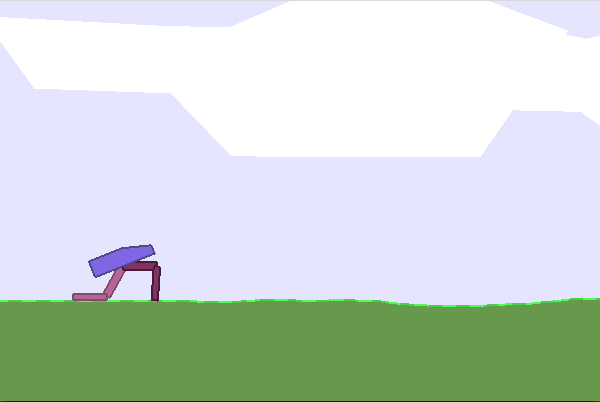
\includegraphics[scale=0.5]{img/robot_walk.png}
     \caption{Robô bípede andando pelo cenário}
     \label{fig:robotwalk}
\end{figure}

\section{Conclusão}

\hspace{1cm}Enfim, o trabalho foi interessante no ponto de vista de aplicação dos conhecimentos sobre algoritmo gênetico obtidos na disciplina. Também vale ressaltar a importância do aprendizado... 


\end{document}
